\documentclass[10pt,letterpaper]{article}
\RequirePackage{amsthm,amssymb,amsmath,graphicx}
\RequirePackage[top=2cm, bottom=2cm, left=2.5cm, right=3cm]{geometry}
\usepackage{caption}
\usepackage{subcaption}
\usepackage[pagebackref=false,colorlinks,linkcolor=black,citecolor=magenta]{hyperref}
\RequirePackage{MnSymbol}
\newcommand{\eqn}[2]{
\begin{equation}
\begin{split}
#1
\label{#2}
\end{split}
\end{equation}
}
%%%%%%%%%%%%%

%       \eqn{
%       x=x^2
%       }{label}

%%%%%%%%%%%%%
\newcommand{\feqn}[2]{
\begin{tcolorbox}[width=7in, colback=white]
\begin{equation}
\begin{split}
#1
\label{#2}
\end{split}
\end{equation}
\end{tcolorbox}
}
%%%%%%%%%%%%%%%
\newcommand{\hl}{
\begin{center}
\line(1,0){450}
\end{center}}
\setlength{\parindent}{0pt}
\newcommand{\nl}{\newline\newline}
\newcommand{\pic}[1]{
\begin{center}
\includegraphics[width=130mm]{#1}
\end{center}
}
%\settextfont{B Nazanin}
\usepackage{lipsum}
\begin{document}
\Large
\begin{center}
The solution of assignment \#6 of the \textbf{ComNet} course
\end{center}
1) a. In the steps of discover and offer, the IP address is not allocated to the newly arrived user, so the broadcast IP address is used to make sure the proper user receives the DHCP response (note that we do not know the IP address of the DHCP server yet).

In the step of request, note that we might have more than one DHCP server present in the network and so we must address all of them.

In the step of ACK, we might have many users requesting for an IP address, so we still need to use a broadcast IP address.

b. The one destined for destination host 11, experiences ICMP type 3 and code 7. The other one, experiences ICMP type 11 and code 0.
\newline\newline
2)
a. 256 users can connect to the first-hop router, of which 3 are not available for allocation to the router, the DHCP server and the network address. Hence, 253 users can connect to the NAT (if you obtained a different answer, fully describe why).

b. Blobking does not occur if we have at most $5$ users simultaneously requesting. Hence, the blocking probability becomes
\eqn{
P_b&=p^6(1-p)+p^7(1-p)+p^8(1-p)+\cdots
\\&=(1-p){p^6\over 1-p}
\\&=p^6<2\times 10^{-5}
}{}
therefore
$$
p<0.1648
$$
\newline\newline
Q3) 
a. The nodes can recognize the presence o each other in two ways: first, they ping each of the other nodes and wait for the response. Second, each node, determines the other nodes presence by their arrived pings. In this scenario, pinging the other nodes and waiting for their response to echo back, takes time as twice as the case where the other node starts a pinging.  For this reason, it is rational to consider the second way of recognition as having the minimum time. Also, since the network is symmetric, we only consider the nodes 2,3,5.

For node $2$, the delay of recognition is

$0.5$msec for nodes 1,3,5

$1$msec for node 4

$1.5$msec for node 6

For node $3$, the delay of recognition is

$0.5$msec for nodes 1,2,4

$1$msec for nodes 5,6

Hence the total delay is $1.5$ msec.

b.
\begin{center}
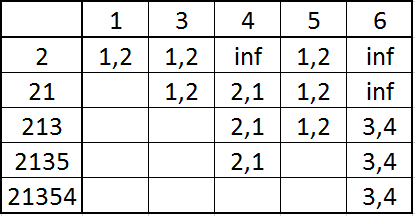
\includegraphics[width=70mm]{Table.png}
\end{center}

Q4) a) The x's distance from u, w and y is 7, 2 and 4, respectively.
\newline\newline
b and c) for any link cost change such that the path or the cost changes, x will inform its neighbors. For example, if $c(x,w)$ is increased (to 3,4,...) or $c(x,y)$ is decreased to less than 1, node x will inform its neighbors, otherwise no information is sent.
\end{document}